\documentclass[12pt, titlepage]{article}

\usepackage{booktabs}
\usepackage{tabularx}
\usepackage{hyperref}
\hypersetup{
    colorlinks,
    citecolor=black,
    filecolor=black,
    linkcolor=red,
    urlcolor=blue
}
\usepackage[round]{natbib}

%% Comments

%\usepackage{color}
\usepackage[dvipsnames]{xcolor}

\newif\ifcomments\commentstrue

\ifcomments
\newcommand{\authornote}[3]{\textcolor{#1}{[#3 ---#2]}}
\newcommand{\todo}[1]{\textcolor{red}{[TODO: #1]}}
\else
\newcommand{\authornote}[3]{}
\newcommand{\todo}[1]{}
\fi

\newcommand{\wss}[1]{\authornote{blue}{SS}{#1}}
\newcommand{\an}[1]{\authornote{magenta}{Author}{#1}}
\newcommand{\meow}[1]{\authornote{Orchid}{JG}{#1}}


% jen things
\usepackage{graphicx} % for pictures
\usepackage{float} % for using [H] in pictures etc.
%% Common Parts

\newcommand{\progname}{Kaplan}

\usepackage{chngpage} % for stretching margins around large tables
\usepackage{listings} % for code lstlisting

\begin{document}

\title{Test Report: Kaplan} 
\author{Jen Garner}
\date{\today}
	
\maketitle

\pagenumbering{roman}

\section{Revision History}

\begin{tabularx}{\textwidth}{p{3cm}p{2cm}X}
\toprule {\bf Date} & {\bf Version} & {\bf Notes}\\
\midrule
December 11, 2018 (Tuesday) & 1.0 & first report \\
\bottomrule
\end{tabularx}

~\newpage

\section{Symbols, Abbreviations and Acronyms}

\renewcommand{\arraystretch}{1.2}
\begin{tabular}{l l} 
  \toprule		
  \textbf{symbol} & \textbf{description}\\
  \midrule 
  T & Test\\
  SMILES & Simplified molecular-input line-entry system \\
  VMD & Visual Molecular Dynamics \\
  IDE & integrated development environment \\
  \bottomrule
\end{tabular}\\

\newpage

\tableofcontents

\listoftables %if appropriate

\listoffigures %if appropriate

\newpage

\pagenumbering{arabic}

This document discusses the results of the unit testing that took place for the 
\progname{} program. The testing was based on the UnitVnVPlan document that can 
be found in the github repository under docs/VnVPlan/UnitVnVPlan. 
\url{https://github.com/PeaWagon/Kaplan}. This report is a partner to the 
System VnV Report that is located in the docs/VnVReport/SystVnVReport directory.

\section{Unit Testing}

During testing, an assertion error was raised when the num\_atoms and size of 
the parser.coords attribute was found to be non-equal. This led to the 
discovery that SMILES strings are case sensitive. The verification of the 
mol\_input module had to be changed to accommodate this discovery. Previously, 
all input was changed to lowercase to avoid case-sensitivity-related errors 
(such as trivial matching errors raised by an incorrect case). Now, all input 
except the SMILES string is changed to lowercase.

Also during testing, an error was found in the vetee program for the write\_xyz 
method of the Xyz class. The method was missing a newline character, and so all 
of the coordinates were being incorrectly written to one line. A new issue was 
raised in the vetee repository on github, and the co-author Kumru Dikmenli was 
able to make a new pypi package with the newline character included. Now the 
output for \progname{} is computer-readable (tested using Visual Molecular 
Dynamics - VMD). See Figure \ref{vmd-figure} for an example of the geometry 
generated with a kaplan output xyz file.

When the tests were run, there would be constant convergence issues from the 
psi4 package. To get around this issue, if a calculation did not work 
(regardless of the error message), the energy would be set to zero. Therefore, 
a more in depth investigation is needed into the types of errors raised by 
psi4, and when they might actually be errors (instead of just convergence 
problems caused by really poor geometry specification).

From the Travis build (see 
\url{https://travis-ci.org/PeaWagon/Kaplan/builds/465876614}), the unit tests 
that have been written thus far have all passed (see Table \ref{trace-MT}). 
Since not all of the unit tests have been written, this measure of success is 
minimal (see the Appendix \ref{report-appendix} for details on which exact 
tests were run). The linters, on the other hand, are causing the Travis build 
to fail as they are not satisfied with the current state of the code. Mainly, 
the errors are coming from incorrect whitespace and missing docstrings. The 
author plans on addressing these problems by opening the code using the PyCharm 
IDE (integrated development environment). The author can use PyCharm to 
automatically highlight all of the linting errors such that they can be fixed. 
A search will also be done to find such tools online (so they don't have to be 
fixed manually) if PyCharm cannot automatically fix the linting problems. The 
docstrings for the modules also have to be written.

\section{Automated Testing}

An example of some of the output can be found in the kaplan/kaplan\_output 
directory of the repository on github \url{https://github.com/PeaWagon/Kaplan}. 
This output was generated by calling the run\_kaplan function in the gac module 
(genetic algorithm control module) with the inputs for 
example2\_mol\_input\_file.txt and example2\_ga\_input\_file.txt (which are 
located in the kaplan/test/testfiles directory).

Based on visual inspection alone of the xyz coordinates, the geometry is 
clearly non-optimal. Since this run only had 5 mating events during which to 
find the optimal solution, the program was not run for long enough such that a 
reasonable geometry could be found.

\begin{figure}
	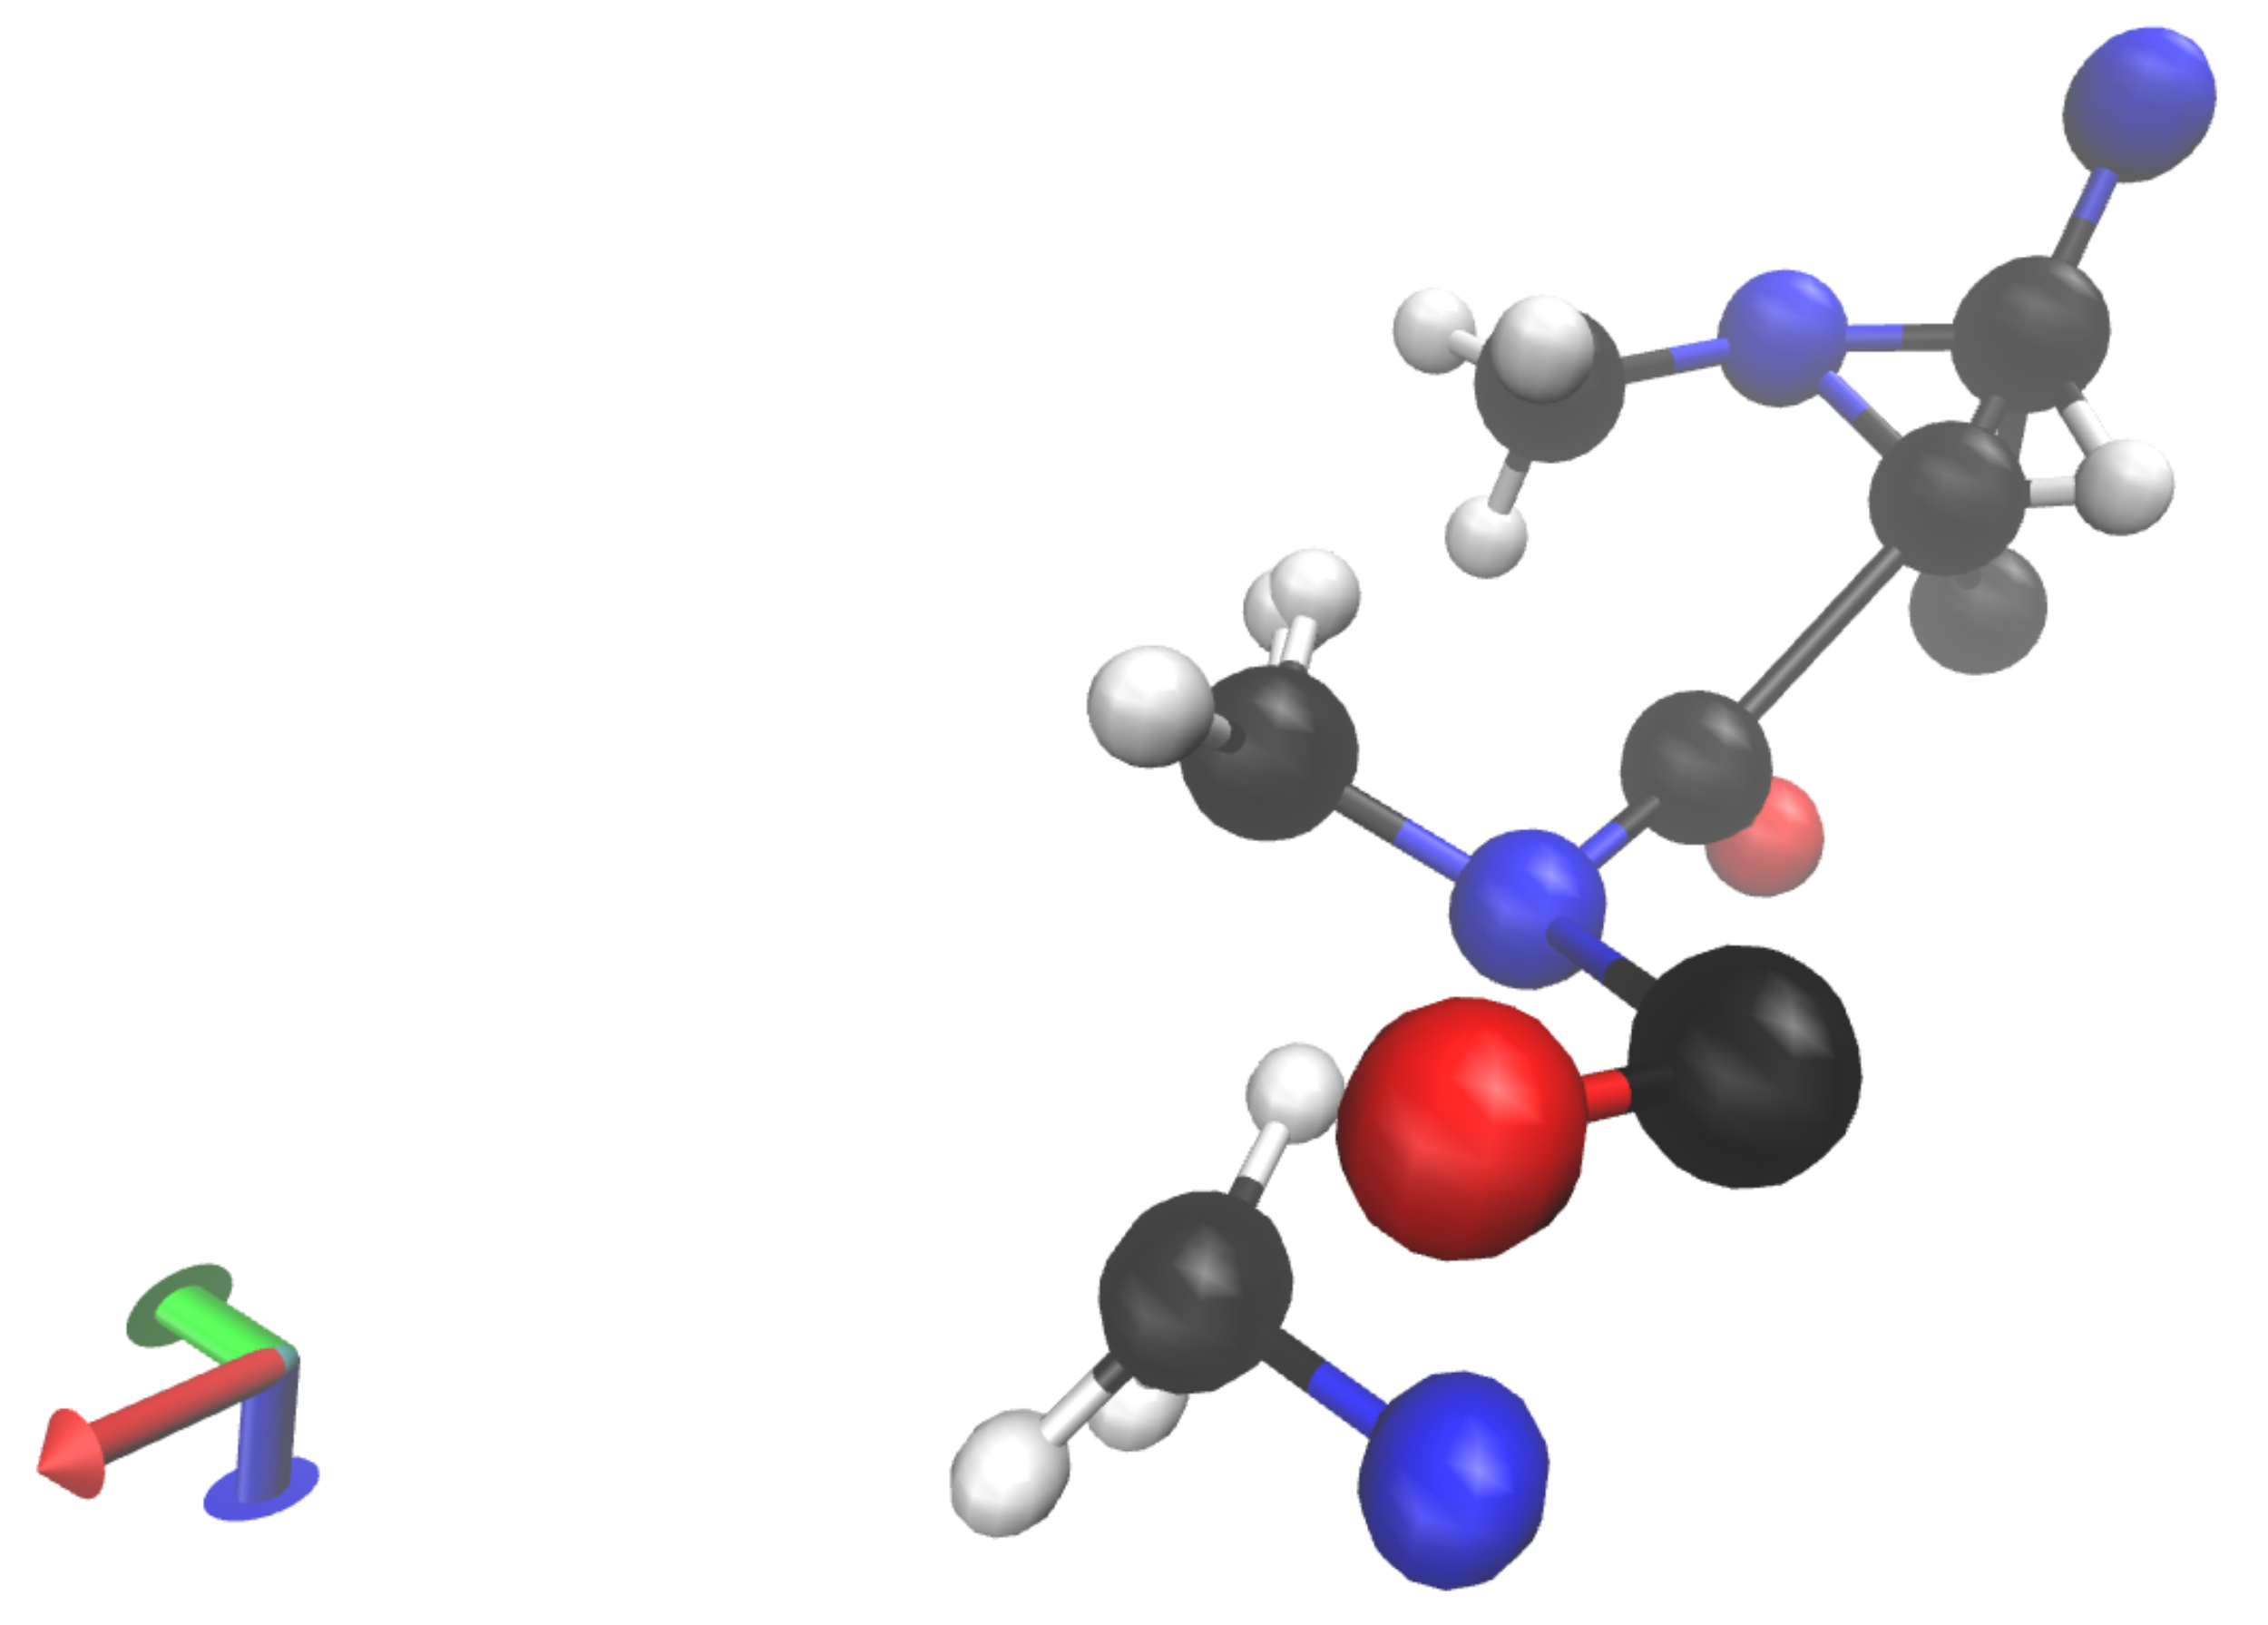
\includegraphics[width=\textwidth]{conf1-caffeine}
	\caption{The output of the caffeine molecule optimization with only 5 
	mating events. Figure generated using VMD (\citet{vmd}, \citet{vmd-pics}).}
\label{vmd-figure}
\end{figure}
		
\section{Trace to Requirements}	

\begin{table}[H]
	\centering
	\begin{tabular}{p{0.2\textwidth} p{0.6\textwidth}}
		\toprule
		\textbf{Req.} & \textbf{Modules}\\
		\midrule
		R1 & mol\_input.py, ga\_input.py \\
		R2 & fitg.py, pmem.py \\
		R3 & fitg.py, rmsd.py, energy.py \\
		R4 & fitg.py, energy.py, geometry.py, mol\_input.py \\
		R5 & output.py, geometry.py, pmem.py \\
		R6 & Satisfied in kaplan/test/testfiles \\
		R7 & tournament.py, mutations.py, ring.py, gac.py \\
		NFR1 & fitg.py \\
		NFR2 & all modules, but especially gac.py \\
		NFR3 & all modules \\
		NFR4 & mol\_input.py, ga\_input.py \\
		NFR5 & energy.py, rmsd.py, mol\_input.py, output.py \\
		\bottomrule
	\end{tabular}
	\caption{Trace between requirements and modules, with the specific python 
	file names given (as found in the kaplan directory). A similar table is 
	found in the module guide document.}
	\label{trace-RM}
\end{table}	

\section{Trace to Modules}

\begin{table}[H]
\begin{adjustwidth}{-0.7in}{-0.5in}
\begin{center}

	\centering
	\begin{tabular}{p{0.4\textwidth} p{0.25\textwidth} p{0.6\textwidth}}
		\toprule
		\textbf{Module} & \textbf{Test File} & \textbf{Comments} \\
		\midrule
		M1 (Hardware Hiding) & - & Out of scope \\
		M2 (GA Input) & test\_ga\_input.py & complete \\
		M3 (Molecule Input) & test\_mol\_input.py & complete \\
		M4 (GA Control) & test\_gac.py & missing assertions for output 
		generation \\
		M5 ($Fit_G$) & tests-for-energy-summation.ipynb & more tests will be 
		written in test\_fitg.py \\
		M6 (Tournament) & test\_tournament.py & incomplete \\
		M7 (Crossover \& Mutation) & test\_mutations.py & mostly complete \\
		M8 (Ring) & test\_ring.py & complete for current spec \\
		M9 (Pmem) & - & test will be written in test\_pmem.py \\
		M10 (Output) & - & test will be written in test\_output.py, tests by 
		visual inspection have been done \\
		M11 (Geometry) & test\_geometry.py and pybel-xyz-zmatrix.ipynb & 
		incomplete \\
		M12 (Energy) & tests-for-energy-summation.ipynb and 
		test\_avail\_psi4.ipynb & incomplete \\
		M13 (RMSD) & rmsd-tests-for-hydrogen.ipynb and test\_rmsd.py & mostly 
		complete (visual inspection still needed) \\
		\bottomrule
	\end{tabular}
	\caption{Trace between modules and tests, with the specific python 
		file names given (as found in the kaplan/test directory), or (if no 
		python test was written) a comment or reference to a jupyter notebook 
		(located in the kaplan/test/jupyter-notebooks directory).}
	\label{trace-MT}

\end{center}
\end{adjustwidth}
\end{table}	

\section{Code Coverage Metrics}

See the System VnV Plan for code coverage, or see the Travis build at this 
link: \url{https://travis-ci.org/PeaWagon/Kaplan/builds/465876614}.

\bibliographystyle {plainnat}

\bibliography {../../../ReferenceMaterial/References}

\section{Appendix}\label{report-appendix}

Here is a list of the tests that have been run for \progname{} using nosetests.

\begin{lstlisting}
kaplan.test.test_generate_children ... ok
kaplan.test.test_run_kaplan ... ok
kaplan.test.test_calc_rmsd ... ok
kaplan.test.test_generate_parser ... ok
kaplan.test.test_Ring ... ok
kaplan.test.test_run_tournament ... ok
kaplan.test.test_read_ga_input ... ok
kaplan.test.test_read_mol_input ... ok
kaplan.test.test_select_pmems ... ok
kaplan.test.test_get_zmatrix_template ... ok
kaplan.test.test_select_parents ... ok
kaplan.test.test_update_zmatrix ... ok
kaplan.test.test_verify_ga_input ... ok
kaplan.test.test_verify_mol_input ... ok
kaplan.test.test_zmatrix_to_xyz ... ok
kaplan.test.test_Ring_fill ... ok
kaplan.test.test_Ring_getitem ... ok
kaplan.test.test_ga_input.test_read_ga_input ... ok
kaplan.test.test_ga_input.test_verify_ga_input ... ok
kaplan.test.test_gac.test_run_kaplan ... ok
kaplan.test.test_geometry.test_generate_parser ... ok
kaplan.test.test_geometry.test_get_zmatrix_template ... ok
kaplan.test.test_geometry.test_update_zmatrix ... ok
kaplan.test.test_geometry.test_zmatrix_to_xyz ... ok
kaplan.test.test_mol_input.test_read_mol_input ... ok
kaplan.test.test_mol_input.test_verify_mol_input ... ok
kaplan.test.test_mutations.test_generate_children ... ok
kaplan.test.test_ring.test_Ring ... ok
kaplan.test.test_ring.test_Ring_fill ... ok
kaplan.test.test_ring.test_Ring_getitem ... ok
kaplan.test.test_ring.test_Ring_setitem ... ok
kaplan.test.test_ring.test_Ring_update ... ok
kaplan.test.test_rmsd.test_calc_rmsd ... ok
kaplan.test.test_tournament.test_run_tournament ... ok
kaplan.test.test_tournament.test_select_pmems ... ok
kaplan.test.test_tournament.test_select_parents ... ok
\end{lstlisting}

\end{document}